%%%%%%%%%%%%%%%%%%%%%%% file template.tex %%%%%%%%%%%%%%%%%%%%%%%%%
%
% This is a general template file for the LaTeX package SVJour3
% for Springer journals.          Springer Heidelberg 2010/09/16
%
% Copy it to a new file with a new name and use it as the basis
% for your article. Delete % signs as needed.
%
% This template includes a few options for different layouts and
% content for various journals. Please consult a previous issue of
% your journal as needed.
%
%%%%%%%%%%%%%%%%%%%%%%%%%%%%%%%%%%%%%%%%%%%%%%%%%%%%%%%%%%%%%%%%%%%
%
% First comes an example EPS file -- just ignore it and
% proceed on the \documentclass line
% your LaTeX will extract the file if required
\begin{filecontents*}{example.eps}
%!PS-Adobe-3.0 EPSF-3.0
%%BoundingBox: 19 19 221 221
%%CreationDate: Mon Sep 29 1997
%%Creator: programmed by hand (JK)
%%EndComments
gsave
newpath
  20 20 moveto
  20 220 lineto
  220 220 lineto
  220 20 lineto
closepath
2 setlinewidth
gsave
  .4 setgray fill
grestore
stroke
grestore
\end{filecontents*}
%
\RequirePackage{fix-cm}
%
%\documentclass{svjour3}                     % onecolumn (standard format)
%\documentclass[smallcondensed]{svjour3}     % onecolumn (ditto)
\documentclass[smallextended]{svjour3}       % onecolumn (second format)
%\documentclass[twocolumn]{svjour3}          % twocolumn
%
\smartqed  % flush right qed marks, e.g. at end of proof
%
\usepackage{graphicx}
\usepackage{epstopdf}
%
% \usepackage{mathptmx}      % use Times fonts if available on your TeX system
%
% insert here the call for the packages your document requires
%\usepackage{latexsym}
% etc.
%
% please place your own definitions here and don't use \def but
% \newcommand{}{}
%
% Insert the name of "your journal" with
% \journalname{myjournal}
%
\begin{document}

\title{Data Paper%\thanks{Grants or other notes
%about the article that should go on the front page should be
%placed here. General acknowledgments should be placed at the end of the article.}
}
%\subtitle{Do you have a subtitle?\\ If so, write it here}

%\titlerunning{Short form of title}        % if too long for running head

\author{First Author         \and
        Second Author %etc.
}

%\authorrunning{Short form of author list} % if too long for running head

\institute{F. Author \at
              first address \\
              Tel.: +123-45-678910\\
              Fax: +123-45-678910\\
              \email{fauthor@example.com}           %  \\
%             \emph{Present address:} of F. Author  %  if needed
           \and
           S. Author \at
              second address
}

\date{Received: date / Accepted: date}
% The correct dates will be entered by the editor


\maketitle

\begin{abstract}
Insert your abstract here. Include keywords, PACS and mathematical
subject classification numbers as needed.
\keywords{First keyword \and Second keyword \and More}
% \PACS{PACS code1 \and PACS code2 \and more}
% \subclass{MSC code1 \and MSC code2 \and more}
\end{abstract}

\section{Introduction}\label{intro}
Text with citations \cite{RefB} and \cite{RefJ}.

\section{Background} \label{sec:1}


\section{Data Collection}\label{sec:2}

\subsection{Hardware Setup}

% For one-column wide figures use
\begin{figure}
  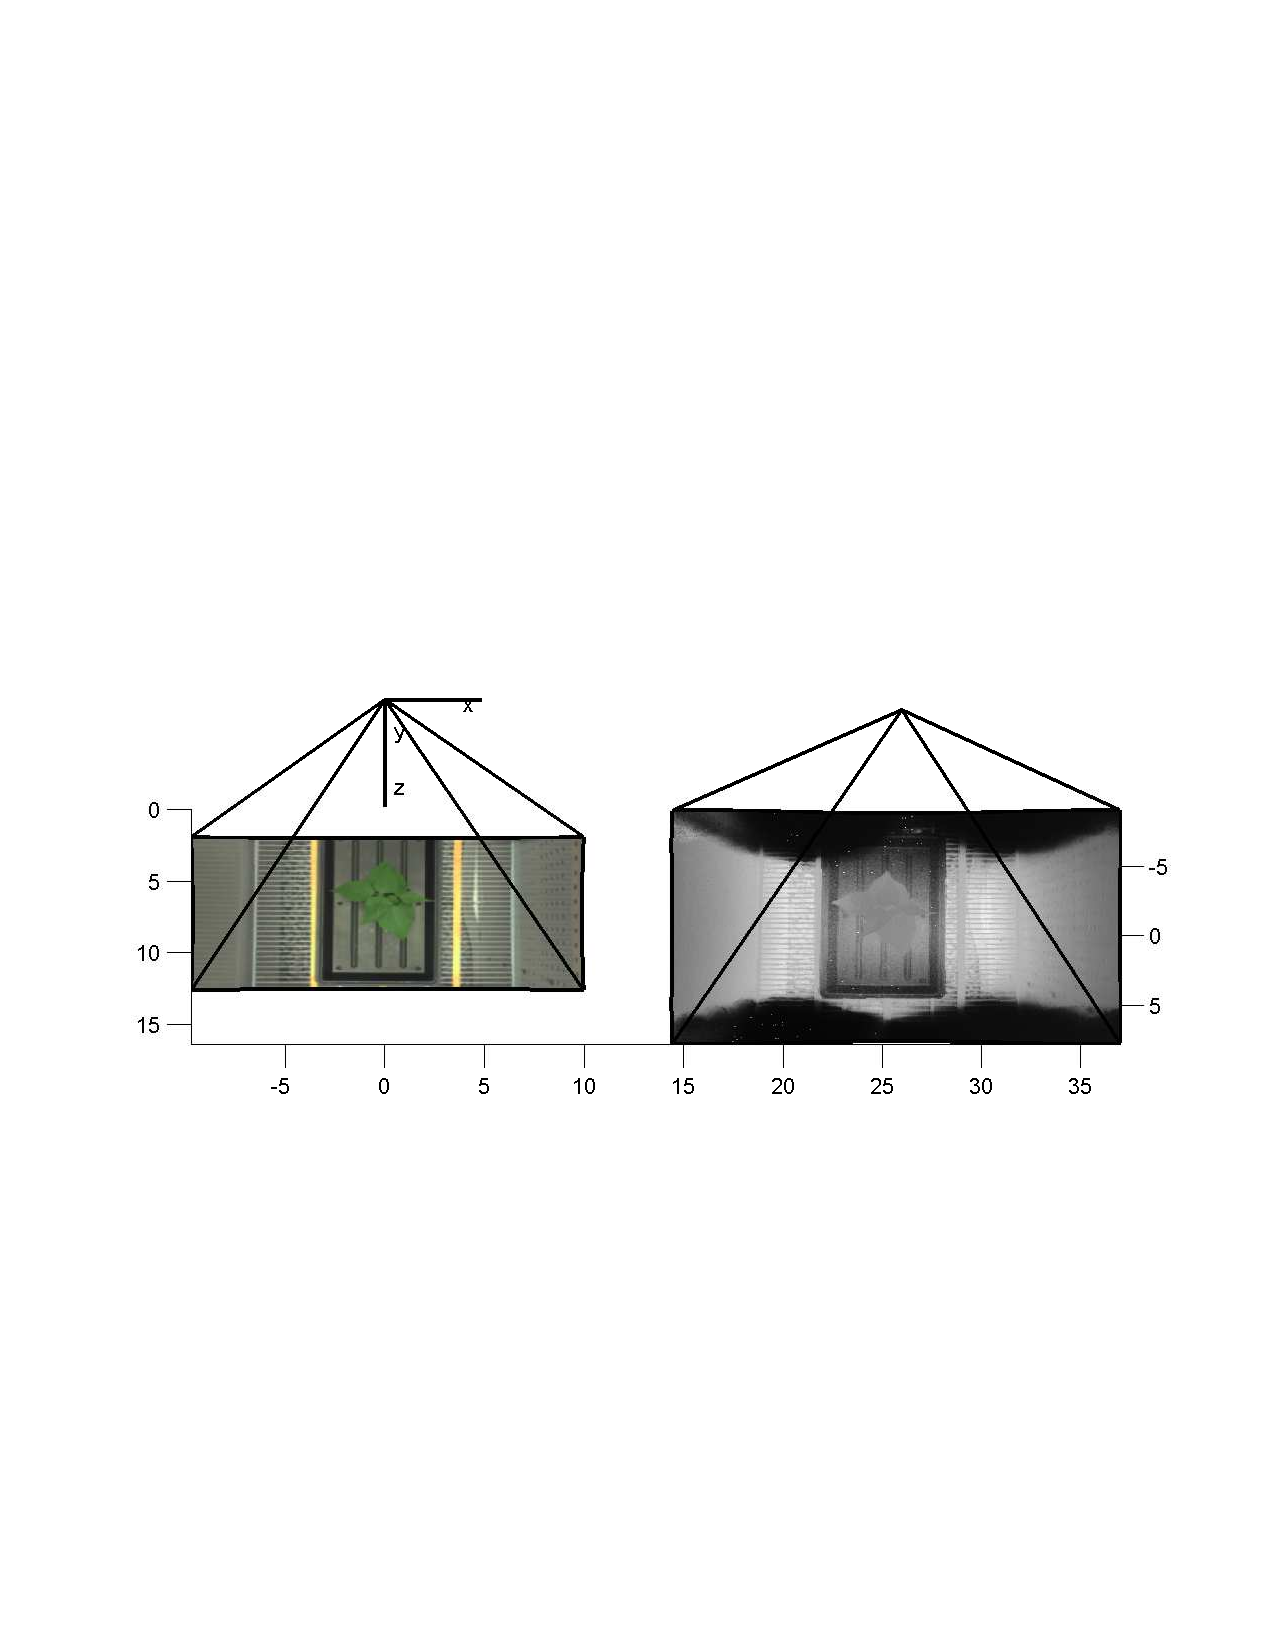
\includegraphics[width=9cm,trim=20 240 20 300,clip]{Figures/CameraConfiguration}
\caption{A plot of the three cameras showing their relative configuration and fields of view as obtained through calibration.  Units are in mm.  In the center is the color camera, and its optical center defines the world coordinate system.  On the right is the depth camera.  Its points are projected into the world coordinate system.  On the left is the fluorescent and IR camera.}
\label{fig:CameraConfiguration} 
\end{figure}

\subsection{Image Accusation}

\subsection{Image Calibration}

\subsection{Creative Senz3D}

The depth and color images were collected using a Creative Senz3D sensor.  This section describes characterizes the data from this sensor, particularly the depth data.  The sensor contains both a $1280 \times 720$ color camera directed parallel to, and separated by roughly 25 mm from, a depth camera which has resolution of $320\times240$ pixels.  The depth sensor uses a flash near IR illuminator and measures the time-of-flight of the beam at each pixel to obtain dense depth estimates along with an IR reflectance at each pixel.    

There are a number of limitations to the depth sensor including sources of depth error.  The primary measurement limit on the range-to-target is the strength of the reflected beam. Hence dark, matt surfaces are measured reliably only at close range on the order of 20 or 30cm.  Highly reflective surfaces also pose problems with direct reflections leading to saturation and highly unreliable depths.  In addition reflective surfaces at grazing angles are less reliably measured as little signal is reflected.  Hence in our data portions of the chamber floor visible in Fig.~\ref{fig:CameraConfiguration} are highly reflective and have incorrect depths.  Fortunately the primary goal of the depth measurements are to obtain leaf depths, and plants provide good, roughly Lambertian reflections of IR CITE{}.  Thus For these reasons the non-leaf depth pixels in the 3D data are unreliable and should be ignored.  Another limitation is that the IR illuminator is slightly offset on the left of the sensor and this results in shadows to the right of some objects, as well as mixed pixels on depth discontinuities.  Both of these can be readily detected as large standard deviations in the depth image.

\subsubsection{Sensor Calibration}

A checkerboard pattern was used to calibrate all three cameras to obtain both intrinsic and extrinsic parameters.  While the checkerboard pattern is not visible as variations in depth, it is nevertheless observed as variations in the reflected IR image whose pixels correspond to the depth pixels.  This enables the use of Zhang's method CITE{} to calculate the intrinsic parameters including a 2-parameter radial distortion of each camera, as well as a calculation of their relative poses.  The optical center of the color camera is used to define the world coordinates of our data.  The depth values of the depth camera are projected along their pixel rays and then rotated and translated by the pose of the depth camera, and thus recorded as 3D points in the world coordinate system.  Hence it is straight forward to project these points onto any of the three camera images.

\subsubsection{Depth Bias and Noise Characterization}
\label{sec:bias}

We characterized both the bias and the variance of the depth cameras as follows.  A flat printed checkerboard with a surrounding white board was positioned at a large number of poses [How many?] in front of the sensor.  The pose of the checkerboard is calculated in each case using the color and IR reflectance images.  This defines a plane relative to the depth camera which we use to calculate the ground truth depths for each pixel in the depth camera.  At each pose we collect multiple depth images; this provides both a bias and variance measurement for each pixel at multiple depths.

Next we sought to model the depth bias as a linear function of depth.  Two parameters were fit for each pixel (a linear coefficient and an offset).  The results are summarized in Fig.~\ref{fig:Bias}.  [Need more summary here.]

\begin{figure}
  %\includegraphics[]{Figures/}
\caption{Noise and Bias model}
\label{fig:Bias} 
\end{figure}


In the recorded 3D data we subtracted our estimated bias, and averaged five depth images for each record.  Hence the actual depth variance for our data is $1/5$ of the the variances shown in Fig.~\ref{fig:Bias}, and the bias is zero.

Now we noticed that the chamber light shades blocked some of the depth camera field of view, and in doing so reflected some of the IR illumination.  This resulted in a bias shift of [how much?].  We removed this bias shift from the depth data.   

\subsubsection{Data Description}

The data consist of 5 images per hour taken within 10 minutes of each other.  These include the fluorescent image, the IR reflectance image with the same camera, the color image, the 3D-depth and a confidence image.  The 3D-depth image is built from the depth sensor by transforming the points into world coordinates and is expressed in mm.  The confidence image is the standard deviation of the depths pixels.  This is useful for identifying pixels at depth discontinuities which are unreliably detected and result in large standard deviations.  In addition pixels with no response and saturated pixels are marked as high standard deviation. [Got to check this].


\subsection{Image Accusation}

\subsection{Image Calibration}

\section{Image Labeling}

\section{Baseline Performance}

\section{Conclusion}

\paragraph{Paragraph headings} Use paragraph headings as needed.
\begin{equation}
a^2+b^2=c^2
\end{equation}

% For one-column wide figures use
\begin{figure}
% Use the relevant command to insert your figure file.
% For example, with the graphicx package use
  
\includegraphics{example.eps}
% figure caption is below the figure
\caption{Please write your figure caption here}
\label{fig:1}       % Give a unique label
\end{figure}
%
% For two-column wide figures use
\begin{figure*}
% Use the relevant command to insert your figure file.
% For example, with the graphicx package use
  
\includegraphics[width=0.75\textwidth]{example.eps}
% figure caption is below the figure
\caption{Please write your figure caption here}
\label{fig:2}       % Give a unique label
\end{figure*}
%
% For tables use
\begin{table}
% table caption is above the table
\caption{Please write your table caption here}
\label{tab:1}       % Give a unique label
% For LaTeX tables use
\begin{tabular}{lll}
\hline\noalign{\smallskip}
first & second & third  \\
\noalign{\smallskip}\hline\noalign{\smallskip}
number & number & number \\
number & number & number \\
\noalign{\smallskip}\hline
\end{tabular}
\end{table}


%\begin{acknowledgements}
%If you'd like to thank anyone, place your comments here
%and remove the percent signs.
%\end{acknowledgements}

% BibTeX users please use one of
%\bibliographystyle{spbasic}      % basic style, author-year citations
%\bibliographystyle{spmpsci}      % mathematics and physical sciences
%\bibliographystyle{spphys}       % APS-like style for physics
%\bibliography{}   % name your BibTeX data base

% Non-BibTeX users please use
\begin{thebibliography}{}
%
% and use \bibitem to create references. Consult the Instructions
% for authors for reference list style.
%
\bibitem{RefJ}
% Format for Journal Reference
Author, Article title, Journal, Volume, page numbers (year)
% Format for books
\bibitem{RefB}
Author, Book title, page numbers. Publisher, place (year)
% etc
\end{thebibliography}

\end{document}
% end of file template.tex

